Esta seção tem como objetivo detalhar as ferramentas escolhidas pela equipe para o desenvolvimento do projeto. Abaixo estão descritas as informações referentes ao repositório do código-fonte, o banco de dados utilizado, a arquitetura do sistema, os protótipos das telas e as tecnologias adotadas.

\subsection{Repositório do Código-Fonte do Projeto} 
O repositório responsável por armazenar e manter o controle de versão do código-fonte do projeto está disponível para consulta no seguinte link: 
\href{https://tools.ages.pucrs.br/salespilot}{\textit{Repositório do Código Fonte}}

\subsection{Banco de Dados Utilizado}
Para o banco de dados, os colegas de \ac{ages} II e III optaram pela utilização do PostgreSQL 16 \cite{PostgreSQL} devido principalmente a sua boa reputação, robustez e alta confiabilidade, sendo executado em um \textit{container} Docker. O versionamento do \textit{schema} é gerenciado pelo Flyway, responsável por aplicar as \textit{migrations} automaticamente durante a inicialização da aplicação. O banco é composto por dois \textit{schemas}: \textbf{public}, onde residem as tabelas da aplicação, e \textbf{auth}. Para a geração de identificadores únicos, é utilizada a extensão \textbf{pgcrypto}, por meio da função \texttt{gen\_random\_uuid()}.

A modelagem é composta pelas tabelas descritas na Tabela \ref{tab:bd-tabelas}.

\begin{table}[H]
\centering
\small
\caption{Tabelas do banco de dados e suas descrições}
\begin{tabular}{|l|p{8.5cm}|}
\hline
\textbf{Tabela} & \textbf{Descrição} \\
\hline
companies & Empresas cadastradas na plataforma \\
\hline
subscription\_plans & Planos de assinatura disponíveis \\
\hline
company\_subscriptions & Associação entre empresas e planos \\
\hline
collaborators & Colaboradores (gestores e vendedores) vinculados a empresas \\
\hline
prompt & \textit{Prompts} de IA vinculados a empresas \\
\hline
prompt\_assignments & Associação entre \textit{prompts} e colaboradores \\
\hline
clients & Clientes vinculados a empresas e colaboradores \\
\hline
meetings & Reuniões realizadas pelos colaboradores com clientes \\
\hline
meeting\_pre\_analysis & Análise pré-reunião gerada pela IA \\
\hline
meeting\_realtime\_insights & \textit{Insights} gerados em tempo real durante a reunião \\
\hline
meeting\_post\_analysis & Análise pós-reunião gerada pela IA \\
\hline
\end{tabular}
\label{tab:bd-tabelas}

\href{https://tools.ages.pucrs.br/salespilot/wiki/-/wikis/Banco-de-Dados}{\textit{Fonte: https://tools.ages.pucrs.br/salespilot/wiki/-/wikis/Banco-de-Dados}}
\end{table}

Em relação aos relacionamentos entre essas tabelas, uma empresa pode ter vários colaboradores, clientes, \textit{prompts} e assinaturas. Um colaborador, por sua vez, pode atender vários clientes, realizar várias reuniões e receber vários \textit{prompts} atribuídos a ele. Já um cliente pode participar de várias reuniões, e cada reunião pode gerar uma análise pré-reunião, diversos \textit{insights} em tempo real e uma análise pós-reunião. Esses relacionamentos estão ilustrados no esquema conceitual apresentado na Figura \ref{fig:bd-esquema-conceitual}.

\begin{figure}[H]
    \centering
    \small
    \caption{Esquema conceitual do banco de dados do SalesPilot}
    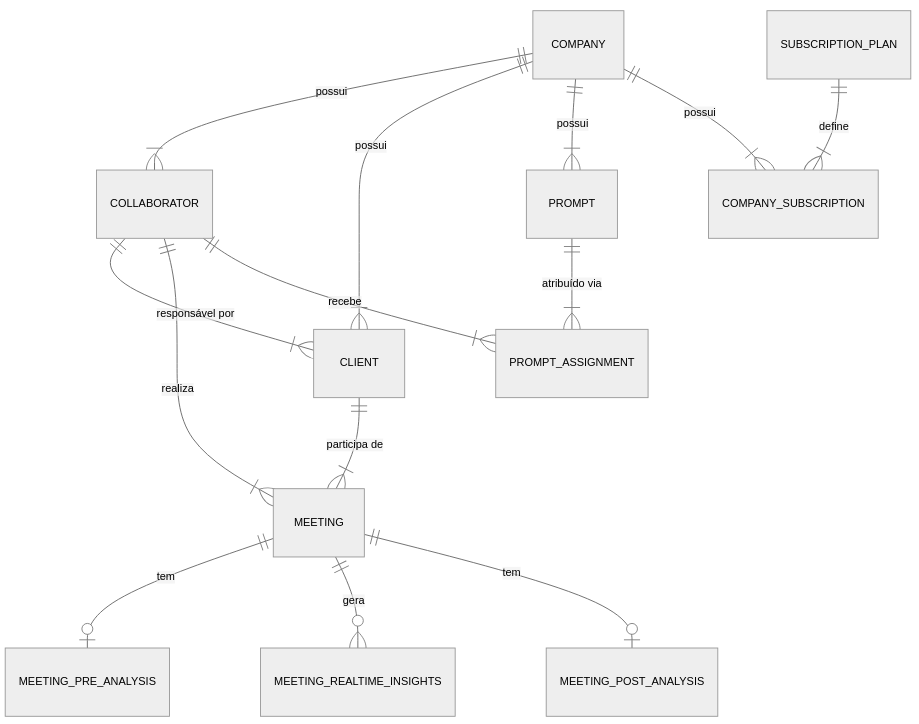
\includegraphics[width=1\linewidth]{conteudo/4 - ages III/conteudo/figures/bd_esquema_conceitual.png}\\
    \label{fig:bd-esquema-conceitual}
    \href{https://tools.ages.pucrs.br/salespilot/wiki/-/wikis/Banco-de-Dados}{\textit{Fonte: https://tools.ages.pucrs.br/salespilot/wiki/-/wikis/Banco-de-Dados}}
\end{figure}

A partir desse esquema conceitual, foi derivado o esquema lógico do banco de dados, apresentado na Figura \ref{fig:bd-esquema-logico}, já contemplando os tipos de dados, chaves primárias e estrangeiras de cada tabela.

\begin{figure}[H]
    \centering
    \small
    \caption{Esquema lógico do banco de dados do SalesPilot}
    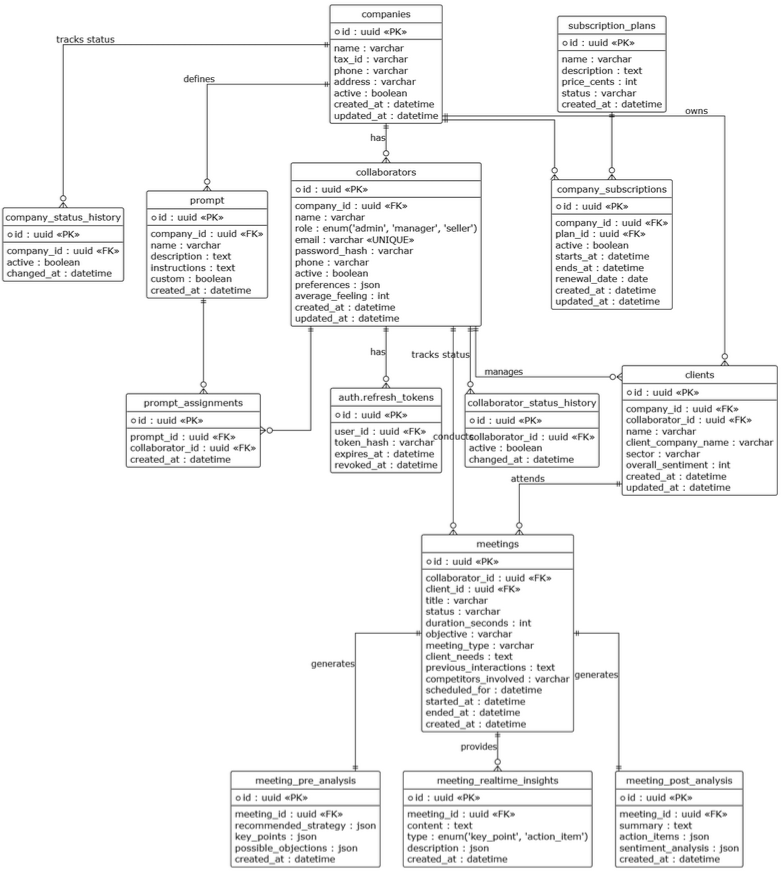
\includegraphics[width=1\linewidth]{conteudo/4 - ages III/conteudo/figures/bd_esquema_logico.png}\\
    \label{fig:bd-esquema-logico}
    \href{https://tools.ages.pucrs.br/salespilot/wiki/-/wikis/Banco-de-Dados}{\textit{Fonte: https://tools.ages.pucrs.br/salespilot/wiki/-/wikis/Banco-de-Dados}}
\end{figure}

Mais detalhes podem ser encontrados aqui:
\href{https://tools.ages.pucrs.br/salespilot/wiki/-/wikis/Banco-de-Dados}{\textit{Banco de Dados}}

\subsection{Arquitetura Utilizada} 
A arquitetura do projeto SalesPilot foi imaginada para ser robusta, modular e escalável, dividindo-se de forma clara entre frontend, backend, banco de dados e infraestrutura em nuvem.

A arquitetura do frontend é composta por React 19 \cite{React}, TypeScript \cite{Typescript} e Vite \cite{Vite} e baseada nos padrões de \textit{feature based architecture} \cite{FeatureBasedArchitecture} e \textit{presentational and container components pattern} \cite{ContainerPresentationalPattern}. O código-fonte principal é organizado dentro do diretório \textbf{src}, que se subdivide em pastas responsáveis por diferentes aspectos do sistema: \textbf{UI} para componentes reutilizáveis entre as diferentes páginas da interface gráfica, \textbf{hooks} para \textit{custom hooks} aproveitados por toda a aplicação, \textit{utils/} para funções de lógica simples e reaproveitável, \textbf{pages} para roteamento, \textbf{store} para o gerenciamento de estados utilizando Zustand e \textbf{services} para a lógica de integração de APIs e funções utilitárias.

Já o backend foi estruturado em Java \cite{Java} com o framework Spring Boot \cite{SpringBoot} e adota uma arquitetura multimódulo Maven fundamentada no Princípio da Inversão de Dependência, onde as dependências apontam estritamente para o interior do sistema isolando as regras de negócio. 

A execução e hospedagem da aplicação são sustentadas por uma infraestrutura provisionada na AWS \cite{AWS}. Os serviços utilizados incluem o Amazon S3 (para armazenamento de exportações CSV geradas pela aplicação), o ECR (repositório para hospedar as imagens dos containers) e o Amazon EFS (para persistência e backup de dados). O processamento computacional foi distribuído em três instâncias EC2:
\begin{itemize}
\item \textbf{EC2 t3.small (GitLab Runner):} responsável por executar os pipelines de CI/CD, realizando o \textit{pull} do repositório GitLab e disparando o \textit{deploy} automatizado.
\item \textbf{EC2 t3.medium (Docker Compose):} atua como a instância principal, hospedando os containers do Front-end, Back-end, PostgreSQL e demais serviços de rastreabilidade.
\item \textbf{EC2 t3.small (SonarQube):} dedicada exclusivamente à análise estática de qualidade de código.
\end{itemize}

\begin{figure}[H]
    \centering
    \small
    \caption{Diagrama de \textit{deploy} da infraestrutura do SalesPilot}
    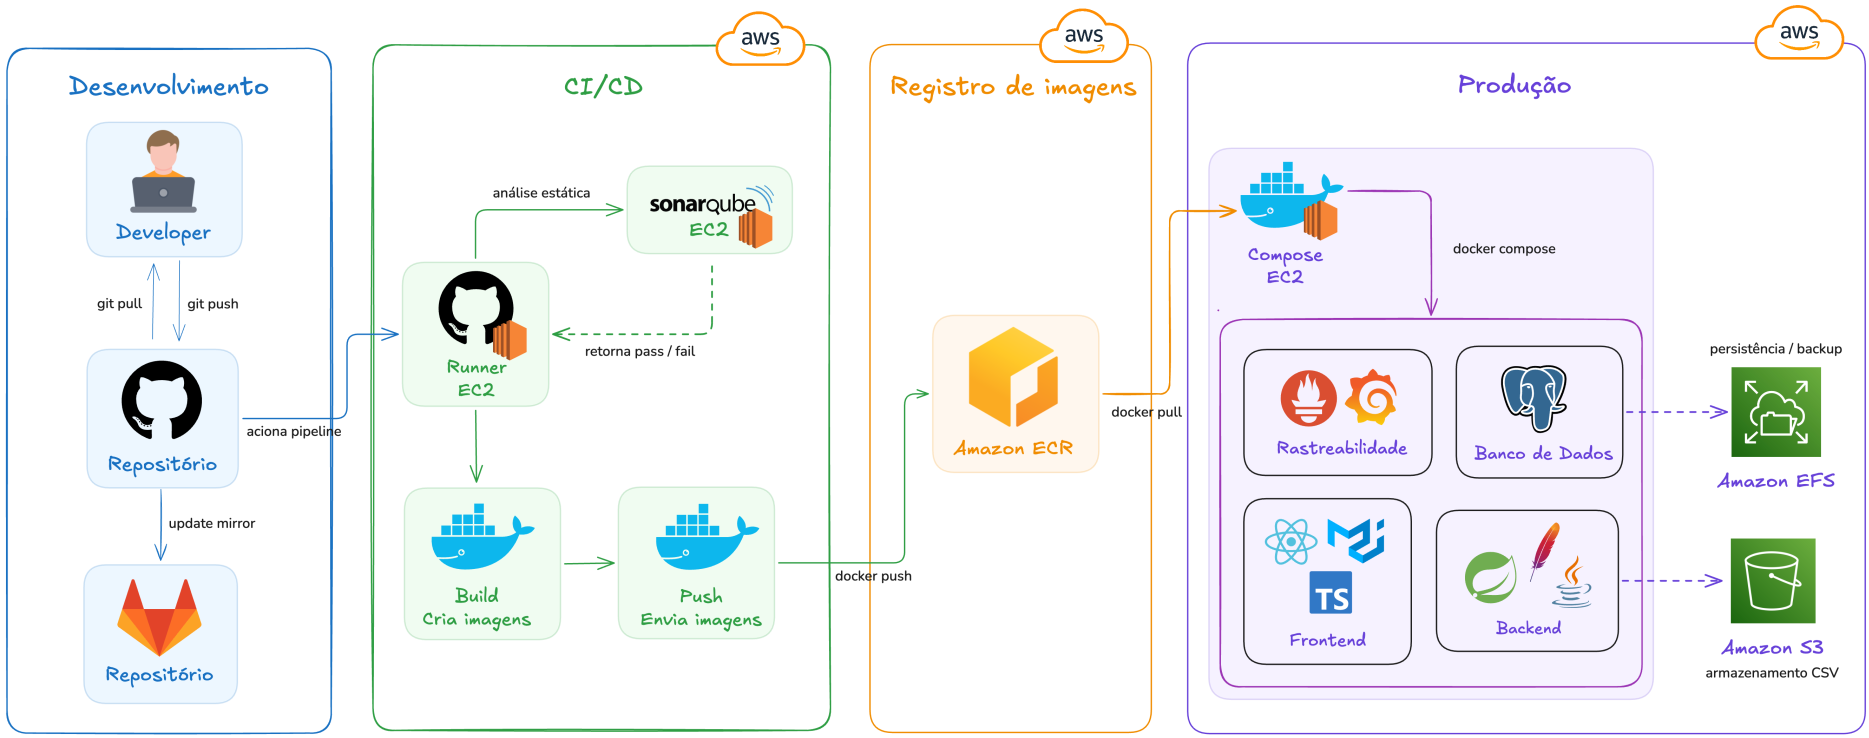
\includegraphics[width=1\linewidth]{conteudo/4 - ages III/conteudo/figures/diagrama_de_deploy_atualizado.png}\\
    \label{fig:diagrama-deploy}
    \href{https://tools.ages.pucrs.br/salespilot/wiki/-/wikis/Arquitetura}{\textit{Fonte: https://tools.ages.pucrs.br/salespilot/wiki/-/wikis/Arquitetura}}
\end{figure}

Mais informações sobre a arquitetura estão disponíveis em:
\href{https://tools.ages.pucrs.br/salespilot/wiki/-/wikis/arquitetura}{\textit{Arquitetura}}

\subsection{Protótipos das Telas Desenvolvidas}
Os protótipos das telas foram criados utilizando a plataforma Figma e os componentes disponibilizados pela comunidade no kit \href{https://www.figma.com/community/file/912837788133317724}{Material UI for Figma}. Os \textit{mockups} de cada tela podem ser visualizados no seguinte link:
\href{https://tools.ages.pucrs.br/salespilot/wiki/-/wikis/design_mockups}{\textit{Protótipo das Telas}}

\begin{figure}[H]
    \centering
    \small
    \caption{Protótipo da tela de \textit{login} do SalesPilot}
    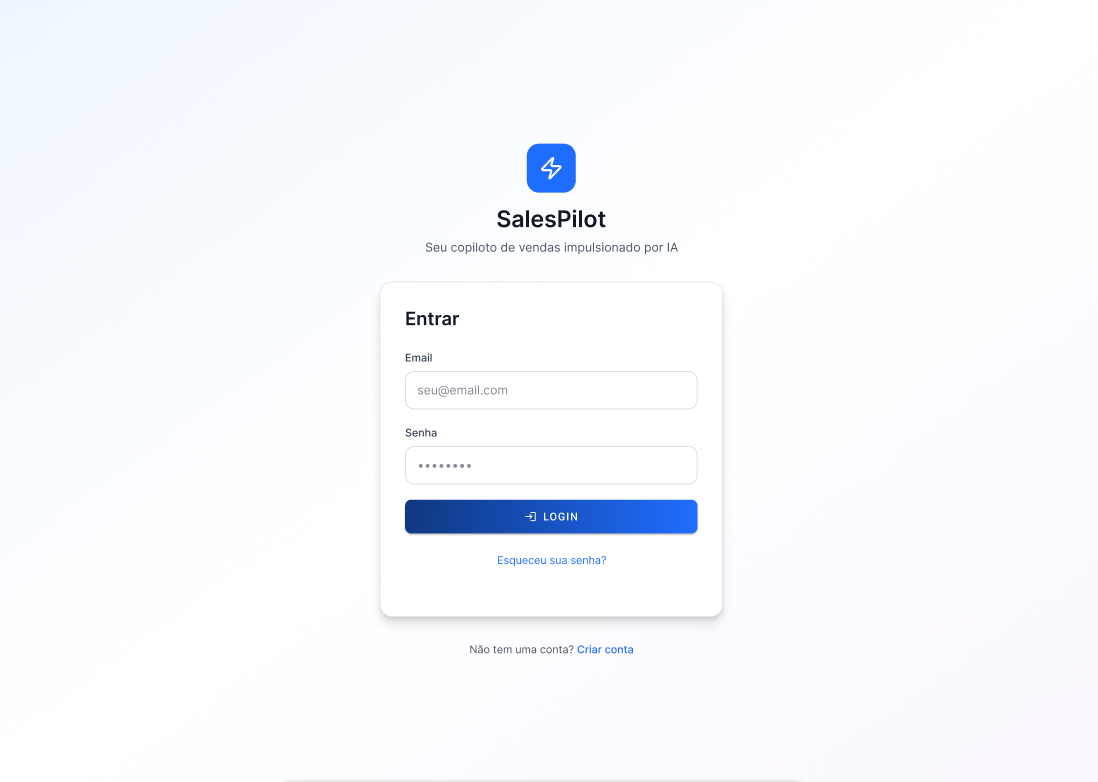
\includegraphics[width=0.5\linewidth]{conteudo/4 - ages III/conteudo/figures/login_mockup.png}\\
    \label{fig:login-mockup}
    \href{https://tools.ages.pucrs.br/salespilot/wiki/-/wikis/Design-Mockups}{\textit{Fonte: https://tools.ages.pucrs.br/salespilot/wiki/-/wikis/Design-Mockups}}
\end{figure}

\subsection{Tecnologias Utilizadas}

Para o frontend, a equipe escolheu trabalhar com TypeScript \cite{Typescript} e React 19 \cite{React}, utilizando Vite \cite{Vite} como ferramenta de automação de build para garantir performance durante o desenvolvimento. A aplicação também utiliza o TanStack Router \cite{TanStackRouter} para o gerenciamento de rotas tipadas e seguras e o TanStack Query \cite{TanStackQuery} para a orquestração do estado do servidor e integração eficiente com o backend. O gerenciamento do estado global da interface é realizado utilizando Zustand \cite{Zustand}, enquanto a validação rigorosa de esquemas de dados e formulários e \textit{schemas} é feita com o uso da biblioteca Zod \cite{Zod}. A interface visual foi desenvolvida com componentes prontos disponibilizados pela biblioteca Material UI (MUI) \cite{MUI}, o que facilitou a implementação do protótipo desenhado no Figma. Para assegurar a confiabilidade e a qualidade do código, foram implementados testes unitários e de componentes utilizando Vitest \cite{Vitest} e React Testing Library \cite{ReactTestingLibrary}, o padrão da indústria para esse tipo de projeto.

No backend, o desenvolvimento foi realizado em Java \cite{Java} com Spring Boot \cite{SpringBoot}, adotando uma estrutura multimódulo Maven \cite{Maven} que segue princípios de arquitetura modular e inversão de dependência para isolar as regras de negócio de detalhes técnicos. O banco de dados escolhido foi o PostgreSQL \cite{PostgreSQL}. 

A infraestrutura completa da aplicação é mantida na nuvem através da AWS \cite{AWS} utilizando instâncias EC2 para hospedagem dos serviços e do SonarQube \cite{SonarQube}, buckets S3, Amazon ECR para a gestão de imagens de containers e Amazon EFS para a persistência e backup de dados. Mais informações detalhadas sobre as tecnologias e os padrões arquiteturais adotados podem ser consultadas nos guias técnicos e na documentação oficial do repositório, através do link:
\href{https://tools.ages.pucrs.br/salespilot/wiki/-/wikis/arquitetura}{\textit{Tecnologias}}
